\documentclass[a4paper]{article}
\usepackage{MyDocumentSettings}

\begin{document}

\pagecolor{oldlace}

\title{The Picolo project}
\author{Adi Kancherla}
\date{November 26, 2017 \\\hfill \\version 1 (private release) \\\hfill \\Whitepaper for the project can be found here \cite{Picolo_Whitepaper}}

\maketitle

\begin{abstract}
This is a work in progress. Methods and equations presented here will most likely change as the platform evolves. Current thinking towards methods for training AI algorithms that make price predictions for cryptos and take bets from users are presented. AI algorithms used here work on two distinct types of data: unstructured in the form of text and structured in the form of polls and games. While the research on sentiment analysis on unstructured data is vast and several off the shelf solutions are available, we explore an approach based on LSTM networks. For structured data, a novel approach is proposed where the state of the platform (all current bets, buzzing topics, randomly timestamped snapshots of past platform state) is reduced to a “game state” and presented as a Markov Decision Process. Incentive decay functions that govern the payouts made to users for contributing on the platform are discussed. 
\end{abstract}


%-----------------------------------------------------------------------------
%  INTRODUCTION
%-----------------------------------------------------------------------------
\section{Introduction}\label{Sect:Introduction}
Blockchain technology is taking the world by storm and is increasingly capturing people’s attention. The total market cap of all the cryptocurrencies and tokens was about \$4 billion at the beginning of 2017 and has grown close to \$300 billion as of December 2017. It is hard to recall such a rate of growth for any industry in history. Much like a startup company that found viral success, the crypto space has much to deal with the unexpected growth in order to take on traditional asset classes and challenge the status quo. While there are excellent infrastructural projects in the works like plasma \cite{Plasma} for solving scaling issues and filecoin \cite{Filecoin} for solving storage issues, there are few projects that take on the problems experienced by the drivers of this boom: investors. In the accompanying whitepaper \cite{Picolo_Whitepaper} we discussed the problem in greater detail and the solution we are building. This paper details some of the initial thoughts on the implementation and underlying technology for the features presented in the whitepaper. The incentive payout system is partly inspired by concepts from Mechanism design theory \cite{Mechanism_design} while AI algorithms draw upon research in the fields of reinforcement learning techniques \cite{Reinforcement_learning} and artificial neural networks \cite{Artificial_neural_network}.


%-----------------------------------------------------------------------------
%  SECTION _ _ _
%-----------------------------------------------------------------------------
\section{Incentive decay functions}
Incentives are based on different categories of contribution. Two examples of categories are bringing new users to the platform and contributing original content. The incentive amount paid out for a user is dependent on how beneficial the user’s contribution is to the platform relative to other users’ contributions in that category. It is calculated by equation \equref{eq:weighted_incentive}

\begin{equation}
i=(w/W)*(I_c)\label{eq:weighted_incentive}
\end{equation}
where
\begin{description}
\item[~$i$] is the incentive amount paid to the user
\item[~$w$] is the user's contribution
\item[~$W$] is the sum of all contributions on the platform
\item[~$I_c$] is the current incentive constant for category c
\end{description}
For example in user growth category, W is the total number of new users on the platform for time period t and w is the number of new users brought to the platform by the user in the same time period.
Incentive constant for a category can be calculated based on heuristics or a time/value based function. A possible heuristic for the user growth category is that the incentive constant halves for every 50,000 new users and can be calculated by the exponential decay function \equref{eq:exp_decay}

\begin{equation}
p_{k+1}=(1/2)*p_k\label{eq:exp_decay}
\end{equation}
or reformulated as a log linear function \equref{eq:log_exp_decay}
\begin{equation}
\log (p_{k+1})=-\log 2 + \log (p_k)\label{eq:log_exp_decay}
\end{equation}
where
\begin{description}
\item[~$p_{k+1}$] is the incentive amount at time k+1
\item[~$p_k$] is the incentive amount at time k
\item and the number of users at time k+1 is 50,000 more than the users at time k
\end{description}
See figure \figref{fig:inc_dec} for a visualization of how the incentives decrease over time.
\begin{figure}[t] \centering
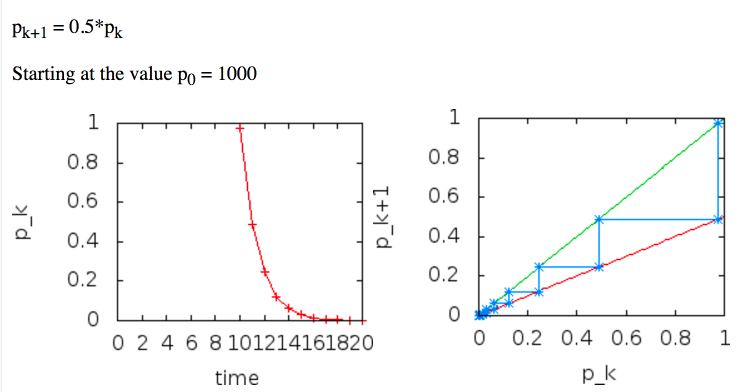
\includegraphics[width=\fscale{1}]{inceDec.png}
\caption{Incentive decay} \label{fig:inc_dec}
\end{figure}


%-----------------------------------------------------------------------------
%  SECTION _ _ _
%-----------------------------------------------------------------------------
\section{AI algorithms}
Lorem ipsum dolor sit amet, consectetur adipisicing elit, sed do eiusmod tempor
incididunt ut labore et dolore magna aliqua. Ut enim ad minim veniam, quis
nostrud exercitation ullamco laboris nisi ut aliquip ex ea commodo consequat.
Duis aute irure dolor in reprehenderit in voluptate velit esse cillum dolore eu
fugiat nulla pariatur. Excepteur sint occaecat cupidatat non proident, sunt in
culpa qui officia deserunt mollit anim id est laborum.

\subsection{Analyzing unstructured data}
LSTM (Long short term memory) is a type of neural network architecture that Analysing structured data

\subsection{Analyzing structured data}
RL methods here



%-----------------------------------------------------------------------------
%  CONCLUSIONS
%-----------------------------------------------------------------------------
\section{Conclusion}
We have proposed initial implementations of the incentive payout system


%-----------------------------------------------------------------------------
%  BIBLIOGRAPHY
%-----------------------------------------------------------------------------
%\pagebreak
\bibliographystyle{unsrt}
\bibliography{./bib/my_bibliography}
\end{document}
